\documentclass[english, a4paper, 11pt]{article}


%%%%%%%%%%% LANGUAGE %%%%%%%%%%%

% For correct hyphenation in swedish
\usepackage[T1]{fontenc}

% For interpreting non-ASCII characters
% \usepackage[utf8]{inputenc}

% International language support
% Fetches language from documentclass options. Most other packages do this as well
\usepackage{babel}


%%%%%%%%%%% FORMAL STUFF %%%%%%%%%%%

% Smaller margins
\usepackage[margin=2.5cm]{geometry}

% Clickable urls
\usepackage[hyphens]{url} % Does not want to be loaded after physics package

% Fancy chapter headers
\usepackage{titlesec}
\titleformat{\chapter}{\normalfont\huge}{\thechapter.}{20pt}{\huge\it}

% Dates & time
\usepackage{datetime} % Useful when referencing websites

% What to display in table of contents
\setcounter{tocdepth}{3}
\setcounter{secnumdepth}{3}

% Lists
\usepackage{enumerate} % Determines the style in which the counter is printed
\usepackage{enumitem} % Provides user control over the layout of the three basic list environments

% Citing & bibliography
\usepackage{csquotes} % For \enquote command for proper quotation marks, also biblatex recommends this
\usepackage[backend=biber, style=numeric, sorting=none]{biblatex}
\bibliography{bibliography} % A file named bibliography.bib containing the bibTeX entries should be placed beside the main.tex file


%%%%%%%%%%% GRAPHICS %%%%%%%%%%%

\usepackage{graphics,color,xcolor}

% Figures
\usepackage{epsfig} % Solves some problems in \includegraphics{<.eps-file>}
\usepackage{graphicx} % More options for \includegraphics
\usepackage{wrapfig} % Figure environment that lets text wrap around figure
\usepackage{float} % Figure placement
\usepackage{caption} % More options for \caption
\usepackage{subcaption} % Subfigures

% Tikz
\usepackage{tikz}
\usepackage{pgf,pgfplots} % Pgfplot
\pgfplotsset{compat=1.15}

% För alduslöv
\usepackage{pifont}


%%%%%%%%%%% PHYSICS %%%%%%%%%%%

% SI units
\usepackage{siunitx}

% Physics macros
\usepackage{physics} % Defines lots of nice commands like \derivative, \norm, \evaluated, etc. It is recommended to use these as much as possible for nice spacing and readable LaTeX code.
\usepackage{braket} % Defines \bra, \ket, \braket, and \set
\usepackage{cancel} % Basically a better version of the \not command
\usepackage{slashed} % For Feynman slash notation
\usepackage{simpler-wick} % Wick contractions (may require sty-file)
\usepackage[compat=1.1.0]{tikz-feynman} % Feynman diagrams (has to be compiled with LuaTeX)


%%%%%%%%%%% CODING %%%%%%%%%%%

% For nice code insertions
\usepackage{listings}
\definecolor{codegreen}{rgb}{0,0.6,0}
\definecolor{codegray}{rgb}{0.5,0.5,0.5}
\definecolor{codepurple}{rgb}{0.58,0,0.82}
\definecolor{backcolour}{rgb}{0.95,0.95,0.92}
\lstdefinestyle{mystyle}{
    backgroundcolor=\color{backcolour},   
    commentstyle=\color{codegreen},
    keywordstyle=\color{magenta},
    numberstyle=\tiny\color{codegray},
    stringstyle=\color{codepurple},
    basicstyle=\ttfamily\footnotesize,
    breakatwhitespace=false,         
    breaklines=true,                 
    captionpos=b,                    
    keepspaces=true,                 
    numbers=left,                    
    numbersep=5pt,                  
    showspaces=false,                
    showstringspaces=false,
    showtabs=false,                  
    tabsize=2
}
\lstset{style=mystyle}


%%%%%%%%%%% MATHEMATICS %%%%%%%%%%%

% AMS packages
\usepackage{amsmath,amsfonts,amsthm,amssymb}

% Sats/bevismiljöer
\iflanguage{swedish}{
    \newtheorem{theorem}{Sats}
    \newtheorem*{theorem*}{Sats}
    \newtheorem{lemma}{Lemma}
    \newtheorem*{lemma*}{Lemma}
    \renewenvironment{proof}{\textit{Bevis.}}{\hfill$\square$}
    \theoremstyle{definition}
    \newtheorem{definition}{Definition}
    \newtheorem*{definition*}{Definition}
}{}
\iflanguage{english}{
    \newtheorem{theorem}{Theorem}
    \newtheorem*{theorem*}{Theorem}
    \newtheorem{lemma}{Lemma}
    \newtheorem*{lemma*}{Lemma}
    \renewenvironment{proof}{\textit{Proof.}}{\hfill$\square$}
    \theoremstyle{definition}
    \newtheorem{definition}{Definition}
    \newtheorem*{definition*}{Definition}
}{}

% Vectors are upright boldface. This definition is better than the physics package's \vectorbold I think.
\renewcommand{\Vec}[1]{{\boldsymbol{\mathrm{#1}}}}
\renewcommand{\vec}[1]{{\boldsymbol{\mathrm{#1}}}}

% Redefine \exp
% Errors occur if this definition is made before some of the packages are loaded
\let\oldexp\exp
\newcommand{\Exp}[1]{\oldexp{#1}}
\renewcommand{\exp}[1]{\mathrm{e}^{#1}}

% Some of my own shorthands for correct spacing in math environments
\newcommand{\from}{\colon} % Proper spacing of colon in functions f: A → B


%%%%%%%%%%% MISCELLANEOUS %%%%%%%%%%%

% In-pdf comments through \todo command
\setlength{\marginparwidth}{2cm} % Silence warning about margin size
\usepackage{todonotes}

% Clickable links and refs
\usepackage[hidelinks]{hyperref} 

% Cleverref automatically detects if you are referencing a figure, table, or equation etc
% Cleverref has to be loaded last I think, after babel and hyperref etc
\usepackage[noabbrev, nameinlink]{cleveref}
\crefname{equation}{}{}
\iflanguage{swedish}{ % Tell cleverref to use Oxford comma
	\newcommand{\creflastconjunction}{, och\nobreakspace}
}{}
\iflanguage{english}{
	\newcommand{\creflastconjunction}{, and\nobreakspace}
}{}


% Tag only referenced equations (this is not an ideal package, as it requires etextools, which is buggy and abandoned by its author)
% \expandafter\def\csname ver@etex.sty\endcsname{3000/12/31}
% \let\globcount\newcount
% \usepackage{autonum}

% For writing \overset{text}&{=} in align environment
\usepackage{aligned-overset} 

\usepackage{simpler-wick} % Wick contractions
\usepackage[compat=1.1.0]{tikz-feynman} % Feynman diagrams

% number sections by a), b), etc & subsections by (i), (ii), etc
\renewcommand{\thesection}{\alph{section})}
\renewcommand{\thesubsection}{\alph{section}.\roman{subsection})}


\title{{\Huge \ding{166}} Quantum Field Theory Problem 4 {\Huge \ding{166}}}
\author{simjac}
\date{\monthname[\the\month] 2020}

\begin{document}

\maketitle


The interactions of pions at low energy can be described by a phenomenological model called the \emph{linear sigma model}. Essentially, this model consists of $N$ real scalar fields coupled by a $\phi^4$ interaction that is symmetric under rotations of the $N$ fields. More specifically, let $\Phi^i(x)$, $i = 1, \dots, N$ be a set of $N$ fields governed by the Hamiltonian
\begin{align}\label{eq:linear_sigma_hamiltonian}
    H = \int \dd^3 \Vec{x} \left( \frac{1}{2} \Pi^2 + \frac{1}{2} (\nabla \Phi)^2 + V(\Phi^2) \right),
\end{align}{}
where $\Phi^2 = \Phi^i \Phi^i$, and
\begin{align}\label{eq:linear_sigma_potential}
    V(\Phi^2) = \frac{1}{2} m^2 \Phi^2 + \frac{\lambda}{4} (\Phi^2)^2
\end{align}{}
is a symmetric function under rotations of $\Phi^i$. For (classical) field configurations of $\Phi^i(x)$ that are constant in space and time, this term gives the only contribution to $H$; hence, $V$ is the field potential energy.

(What does this Hamiltonian have to do with the strong interactions? There are two types of light quarks, $u$ and $d$. These quarks have identical strong interactions, but different masses. If these quarks are massless, the Hamiltonian of the strong interactions is invariant to unitary transformations of the 2-component object $(u, d)$:
\begin{equation*}
    \begin{pmatrix}
        u\\
        d
    \end{pmatrix}{}
    \mapsto
    \Exp{i \Vec{\alpha} \cdot \Vec{\sigma} / 2}
        \begin{pmatrix}
        u\\
        d
    \end{pmatrix}{}.
\end{equation*}{}
This transformation is called an \emph{isospin} rotation. If, in addition, the strong interactions are described by a vector \say{gluon} field (as is true in QCD), the strong interaction Hamiltonian is invariant to the isospin rotations done separately on the left-handed and right-handed components of the quark fields. Thus, the complete symmetry of QCD with two massless quarks is $SU(2) \times SU(2)$. It happens that $SO(4)$, the group of rotations in 4 dimensions, is isomorphic to $SU(2) \times SU(2)$, so for $N = 4$, the linear sigma model has the same symmetry group as the strong interactions.)

\section{}

Analyze the linear sigma model for $m^2 > 0$ by noticing that, for $\lambda = 0$, the Hamiltonian given above is exactly $N$ copies of the Klein-Gordon Hamiltonian. We can then calculate scattering amplitudes as perturbation series in the parameter $\lambda$.

\subsection{}
Show that the propagator is
\begin{equation*}
    \wick{
        \c1 \Phi^i(x) \c1 \Phi^j(y) = \delta^{ij} D_\mathrm{F}(x - y),
    } 
\end{equation*}{}
where $D_\mathrm{F}$ is the standard Klein-Gordon propagator for mass $m$,

\subsection*{Solution}

If $\lambda = 0$, \cref{eq:linear_sigma_hamiltonian} is just the Klein-Gordon Hamiltonian. Using the Peskin and Schroeder equation numbering, we have that
\begin{align*}
	\wick{\c1 \Phi^i(x) \c1 \Phi^j(y)} &:=
	\begin{cases}
		[\Phi^i{}^+(x), \Phi^j{}^-(y)], \quad &x^0 > y^0\\
		[\Phi^i{}^+(y), \Phi^j{}^-(x)], \quad &x^0 < y^0
	\end{cases}\\
	%
	\overset{(4.32)}&{=}
	\int \frac{\dd^3 \vec{p} \,\dd^3 \vec{q}}{(2 \pi)^6} \frac{1}{\sqrt{2 \cdot 2 E_\vec{p} E_\vec{q}}} \left[ a^i_\vec{p}, a^j{}^\dagger_\vec{q} \right]
	\begin{cases}
		\Exp{i(-p^\alpha x_\alpha + q^\alpha y_\alpha)}, \quad &x^0 > y^0\\
		\Exp{i(p^\alpha x_\alpha - q^\alpha y_\alpha)}, \quad &x^0 < y^0
	\end{cases}\\
	%
	\overset{(2.29)}&{=}
	\int \frac{\dd^3 \vec{p} \,\dd^3 \vec{q}}{(2 \pi)^6} \frac{1}{\sqrt{2 \cdot 2 E_\vec{p} E_\vec{q}}} \delta^{ij} (2 \pi)^3 \delta^3(\vec{p} - \vec{q})
	\begin{cases}
		\Exp{i(-p^\alpha x_\alpha + q^\alpha y_\alpha)}, \quad &x^0 > y^0\\
		\Exp{i(p^\alpha x_\alpha - q^\alpha y_\alpha)}, \quad &x^0 < y^0
	\end{cases}\\
	%
	&= \delta^{ij}
	\int \frac{\dd^3 \vec{p}}{(2 \pi)^3} \frac{1}{2 E_\vec{p}}
	\begin{cases}
		\Exp{i p^\alpha (-x + y)_\alpha}, \quad &x^0 > y^0\\
		\Exp{i p^\alpha (x - y)_\alpha}, \quad &x^0 < y^0
	\end{cases}\\
	%
	\overset{(2.50)}&{=}
	\begin{cases}
	D(x - y), \quad &x^0 > y^0\\
	D(x - y), \quad &x^0 < y^0
	\end{cases}\\
	%
	\overset{(2.60)}&{=} D_\mathrm{F}(x - y).
\end{align*}



\subsection{}
and that there is one type of vertex given by
\begin{equation*}
    \feynmandiagram[inline=(o.base), vertical=a to b]{
        o [dot],
        o -- a,
        o -- b,
        o -- c,
        o -- d,
        a [label=$l$],
        b [label=$j$],
        c [label=$k$],
        d [label=$i$],
        a -- [draw=none] b,
        c -- [draw=none] d,
    };
    = -2 i \lambda \left( \delta^{ij} \delta^{kl} +  \delta^{il} \delta^{jk} + \delta^{ik} \delta^{jl} \right).
\end{equation*}{}
(That is, a vertex between two $\Phi^1$:s and two $\Phi^2$:s has the value ($-2 i \lambda$); that between four $\Phi^1$:s has the value ($-6 i \lambda$).)

\subsection*{Solution}
TODO: BOTH ERIC \& ARVID SEEM TO THINK THIS IS TRIVIAL, BUT WHY THO?\\
USE (A.2) FROM PESKIN \& SCHROEDER?




\subsection{}
Compute, to leading order in $\lambda$, the differential cross section $\dd \sigma / \dd \Omega$, in the center-of-mass frame, for the scattering processes
\begin{equation*}
    \Phi^1 \Phi^1 \to \Phi^1 \Phi^2, \quad \Phi^1 \Phi^1 \to \Phi^2 \Phi^2, \quad \textrm{and} \quad \Phi^1 \Phi^1 \to \Phi^1 \Phi^1
\end{equation*}{}
as a function of their center-of-mass energy.


\subsection*{Solution}
\begin{align*}
	\Phi^1 \Phi^1 \to \Phi^1 \Phi^2 : \quad i \mathcal{M} = TODO \implies \left( \frac{\dd \sigma}{\dd \Omega} \right)_\mathrm{CM} = TODO
\end{align*}





\section{}
Now consider the case $m^2 < 0$: $m^2 = -\mu^2$. In this case, $V$ has a local maximum, rather than a minimum, at $\Phi^i = 0$. Since $V$ is a potential energy, this implies that the ground state of the theory is not near $\Phi^i = 0$ but rather is obtained by shifting $\Phi^i$ toward the minimum of $V$. By rotational invariance, we can consider this shift to be in the $N$th direction. Write, then,
\begin{align*}
    \Phi^i(x) &= \pi^i(x), \quad i = 1, \dots, N -1\\
    %
    \Phi^N(x) &= v + \sigma(x),
\end{align*}{}
where $v$ is a constant chosen to minimize $V$. (The notation $\pi^i$ suggests a pion field and should not be confused with a canonical momentum.)

\subsection{}
Show that, in these new coordinates (and substituting for $v$ its expression in terms of $\lambda$ and $\mu$), we have a theory of a massive $\sigma$ field and $N - 1$ \emph{massless} pion fields, interacting through cubic and quartic potential energy terms which all become small as $\lambda \to 0$.

\subsection*{Solution}
As in Home Problem 1 c), we have that
\begin{align*}
	v = \frac{\mu}{\sqrt{\lambda}}
\end{align*}
minimizes the potential. Substituting this and $\Phi^i(x) = (\pi^j(x), v + \sigma(x)), j = 1, \dots, N-1$ into \cref{eq:linear_sigma_potential}, we get (see \cref{fig:linear_sigma_potential_calculation} for this calculation)
\begin{align}\label{eq:linear_sigma_potential_calculation}
	V(\Phi^2) = 
	-\frac{\mu ^4}{4 \lambda }+\sqrt{\lambda } \mu  \sigma ^3+\pi ^2 \sqrt{\lambda } \mu  \sigma +\frac{\lambda  \sigma ^4}{4}+\frac{1}{2} \pi ^2 \lambda  \sigma ^2+\frac{\pi ^4 \lambda }{4}+\mu ^2 \sigma ^2,
\end{align}
where $\pi^2 = \pi^j \pi^j$. We see that the $\sigma$ field has a mass term, $\mu^2 \sigma^2$, while the $\pi$ fields have no mass terms. The fields are also evidently \say{interacting through cubic and quartic potential energy terms which all become small as $\lambda \to 0$} since all those terms have a factor of $\lambda$ or $\sqrt{\lambda}$ in them.
\begin{figure}[h]
	\centering
	\fbox{
		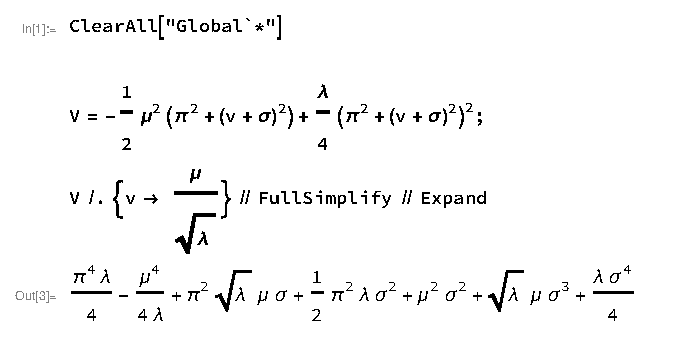
\includegraphics[width=0.9\textwidth]{linear_sigma_potential_calculation.pdf}
	}
	\caption{Mathematica code for \cref{eq:linear_sigma_potential_calculation}. Since everything here commutes, we might as well pretend that everything is c-numbers.}
	\label{fig:linear_sigma_potential_calculation}
\end{figure}{}




\subsection{}\label{sec:b_ii}
Construct the Feynman rules by assigning values to the propagators and vertices:
\begin{align*}
    \wick{\c1{\sigma} \c1{\sigma}} &= 
    \feynmandiagram[small, inline=(a.base), horizontal=a to b]{
        a -- [double distance=1.5pt, with arrow=0.7cm] b,
    };\quad~
    \quad
    \feynmandiagram[small, inline=(o.base), vertical=a to o]{
    	o [dot],
        a -- [double distance=1.5pt] o,
        b -- o,
        c -- o,
        b [label=$i$],
        c [label=$j$]
    };~~~~
    \feynmandiagram[small, inline=(o.base), vertical=a to o]{
    	o [dot],
        a -- [double distance=1.5pt] o,
        b -- [double distance=1.5pt] o,
        c -- [double distance=1.5pt] o,
    };\\
    %
    \wick{\c1\pi^i \c1\pi^j} &= 
    \feynmandiagram[small, inline=(a.base), horizontal=a to b]{
        a -- [fermion] b,
        a [label=$i$],
        b [label=$j$],
    };\quad~
    \feynmandiagram[small, inline=(o.base), vertical=a to b]{
		o [dot],
        a -- o,
        b -- o,
        c -- o,
        d -- o,
        a [label=$l$],
        b [label=$j$],
        c [label=$k$],
        d [label=$i$],
        a -- [draw=none] b,
        c -- [draw=none] d,
    };~~~~
    \feynmandiagram[small, inline=(o.base), vertical=a to b]{
    	o [dot],
        a -- [double distance=1.5pt] o,
        b -- o,
        c -- [double distance=1.5pt] o,
        d -- o,
        b [label=$j$],
        d [label=$i$],
        a -- [draw=none] b,
        c -- [draw=none] d,
    };~~~~
    \feynmandiagram[small, inline=(o.base), vertical=a to b]{
    	o [dot],
        a -- [double distance=1.5pt] o,
        b -- [double distance=1.5pt] o,
        c -- [double distance=1.5pt] o,
        d -- [double distance=1.5pt] o,
        a -- [draw=none] b,
        c -- [draw=none] d,
    };.
\end{align*}

\subsection*{Solution}
$\wick{\c1{\sigma} \c1{\sigma}}$ is just the propagator for a free $\sigma$ particle is,
\begin{align*}
	\wick{\c1{\sigma} \c1{\sigma}}
	= \frac{i}{p^2 - 2 \mu^2}.
\end{align*}
Likewise, $\wick{\c1\pi^i \c1\pi^j}$ is, since the pion is massless, 
\begin{align*}
	\wick{\c1\pi^i \c1\pi^j}
	= \frac{i\delta^{ij}}{p^2}.
\end{align*}

\begin{align}
	\feynmandiagram[small, inline=(o.base), vertical=a to o]{
		o [dot],
		a -- [double distance=1.5pt] o,
		b -- o,
		c -- o,
		b [label=$i$],
		c [label=$j$]
	}; &= -2i\lambda v\delta^{ij}\\
	\feynmandiagram[small, inline=(o.base), vertical=a to o]{
		o [dot],
		a -- [double distance=1.5pt] o,
		b -- [double distance=1.5pt] o,
		c -- [double distance=1.5pt] o,
	}; &= -6i\lambda v\\
	\feynmandiagram[small, inline=(o.base), vertical=a to b]{
		o [dot],
		a -- o,
		b -- o,
		c -- o,
		d -- o,
		a [label=$l$],
		b [label=$j$],
		c [label=$k$],
		d [label=$i$],
		a -- [draw=none] b,
		c -- [draw=none] d,
	}; &= -2 i \lambda \left( \delta^{ij} \delta^{kl} +  \delta^{il} \delta^{jk} + \delta^{ik} \delta^{jl} \right)\\
	\feynmandiagram[small, inline=(o.base), vertical=a to b]{
		o [dot],
		a -- [double distance=1.5pt] o,
		b -- o,
		c -- [double distance=1.5pt] o,
		d -- o,
		b [label=$j$],
		d [label=$i$],
		a -- [draw=none] b,
		c -- [draw=none] d,
	};&= -2i\lambda \delta^{ij}\\
	\feynmandiagram[small, inline=(o.base), vertical=a to b]{
		o [dot],
		a -- [double distance=1.5pt] o,
		b -- [double distance=1.5pt] o,
		c -- [double distance=1.5pt] o,
		d -- [double distance=1.5pt] o,
		a -- [draw=none] b,
		c -- [draw=none] d,
	};&= -6i\lambda
\end{align}





\section{}
\subsection{}
Compute the scattering amplitude for the process
\begin{equation*}
    \pi^i(p_1) \pi^j(p_2) \to \pi^k(p_3) \pi^l(p_4)
\end{equation*}{}
to leading order in $\lambda$. There are now four Feynman diagrams that contribute:
\begin{equation*}
    \feynmandiagram[small, inline=(t.base), vertical=c to d]{
        a -- c,
        b -- c,
        c -- [double distance=1.5pt] d,
        e -- d,
        f -- d,
        c -- [draw=none] t, % t is center point for baseline
        d -- [draw=none] t,
        a [label=$l$],
        b [label=$k$],
        e [label=$j$],
        f [label=$i$],
    };
    +
    \feynmandiagram[small, inline=(c.base), horizontal=c to d]{
        a -- c,
        b -- c,
        c -- [double distance=1.5pt] d,
        e -- d,
        f -- d,
        a -- [draw=none] b,
        e -- [draw=none] f,
        a [label=$i$],
		b [label=$k$],
		e [label=$j$],
		f [label=$l$],
    };
	+
	\feynmandiagram[small, inline=(c.base), horizontal=c to d]{
        a -- [draw=none] c,
		c -- g,
		d -- h,
        b -- [draw=none] c,
        c -- [double distance=1.5pt] d,
        e -- [draw=none] d,
        f -- [draw=none] d,
        c -- f,
		d -- b,
        a -- [draw=none] b,
        e -- [draw=none] f,
		f -- [draw=none] b,
  		g [label=$i$],
		h [label=$j$],
		b [label=$k$],
		f [label=$l$],
    };
	+
	\feynmandiagram[inline=(o.base), vertical=a to b]{
		o -- a,
		o -- b,
		o -- c,
		o -- d,
		a -- [draw=none] b,
		c -- [draw=none] d,
		a [label=$l$],
		b [label=$j$],
		c [label=$k$],
		d [label=$i$],
	};.
\end{equation*}

\subsection*{Solution}
Multiplying the together values we derived in \cref{sec:b_ii} for each vertex, we get
\begin{align*}
	\mathcal{M}_{ij\rightarrow kl} &= -2i\lambda v \delta^{ij} \dfrac{i}{p^2-2\mu^2+i\epsilon} (-2i)\lambda v \delta^{kl} = -4i\lambda^2v^2\delta^{ij}\delta^{kl}\dfrac{1}{p^2-2\mu^2+i\epsilon}\\
	%
	\mathcal{M}_{ik\rightarrow jl} &= -2i\lambda v \delta^{jl} \dfrac{i}{p^2-2\mu^2+i\epsilon} (-2i)\lambda v \delta^{ik}=-4i\lambda^2v^2\delta^{jl}\delta^{ik}\dfrac{1}{p^2-2\mu^2+i\epsilon}\\
	%
	\mathcal{M}_{ij\rightarrow lk} &= -2i\lambda v \delta^{ij} \dfrac{i}{p^2-2\mu^2+i\epsilon} (-2i)\lambda v \delta^{lk}=-4i\lambda^2v^2\delta^{ij}\delta^{lk}\dfrac{1}{p^2-2\mu^2+i\epsilon}\\
	%
	\widetilde{\mathcal{M}}_{ij\rightarrow kl} &= -2 i \lambda \left( \delta^{ij} \delta^{kl} +  \delta^{il} \delta^{jk} + \delta^{ik} \delta^{jl} \right).
\end{align*}




\subsection{}
Show that, at treshold ($\vec{p} = 0$), these diagrams sum to \emph{zero}. (Hint: It may be easiest to first consider the specific process $\pi^1 \pi^1 \to \pi^2 \pi^2$, for which only the first and fourth diagrams are nonzero, before tackling the general case.)






\subsection{}
Show that, in the special case $N = 2$ (1 species of pion), the term of $\mathcal{O}(p^2)$ also cancels.


\subsection*{Solution}



\section{}
Add to $V$ a symmetry-breaking term,
\begin{equation*}
	\Delta V = - a \Phi^N,
\end{equation*}
where $a$ is a (small) constant. (In QCD, a term of this form is produced if the $u$ and $d$ quarks have the same nonvanishing mass.)

\subsection{}
Find the new value of $v$ that minimizes $V$,

\subsection*{Solution}


\subsection{}
and work out the content of the theory about that point.

\subsection*{Solution}


\subsection{}
Show that the pion acquires a mass such that $m^2_\pi \sim a$, 

\subsection*{Solution}


\subsection{}
and show that the pion scattering amplitude at treshold is now nonvanishing and also proportional to $a$.















\end{document}